\clearpage
\subsection{Contributions of thesis}

The goal of the current thesis is to acquire a better understanding of
laser-matter interaction.
More specifically, the
question of \textit{how} the energy is deposited in a nanoscale object
--a rare gas cluster-- by an
ultra-short and ultra-intense laser pulse will be studied. This interaction
largely depends on the specific target material and on the pulse's wavelength
and duration, both defining the interaction regime. A specific regime will
thus be targeted; mainly short wavelengths, from VUV to XUV, as many questions
raising from recent experiments are still debated.

While many tools exist to study laser-mater interaction, only classical
approaches can be considered since a full quantum calculation, even
with some degree of approximations, is not possible. Clusters become
nanoplasmas quite rapidly and have large charge and field fluctuations inside
them. This and their finite nature makes it hard to use tools such as rate
equations to model them. Pure classical simulations allows for relatively large
systems to be simulated and are thus the tool of choice.

\lrnote{also remind me to talk to you about justifications of classical
regmies in plasma physics... we might add that discussion here.}

\subsubsection{Tools}

First, chapter \ref{section:tools} describes the different tools and models
that were developed and implemented to answer our questions. While chapter
\ref{section:tools:md} concentrate on the classical aspect of the problem,
chapter \ref{section:tools:qfdtd} describes in detail a quantum approach that
was used named QFDTD for Quantum Finite-Difference Time-Domain.
Note that all implementations used are original work; all code packages
were developed from scratch by me or under my direction and no external packages
were used. The MD package described in
chapter \ref{section:tools:md} ($\sim$16k lines of code) contains 86~\% of code
written by me, 12~\% by Edward Ackad (postdoctoral fellow) and smaller contributions from
Julien Roy (undergraduate student) during his summer 2012 internship. Furthermore, the QFDTD package
($\sim$16k lines of code) contains 3~\% of code written by Stan Hatko (undergraduate student) while the
rest is my original work. Most tools were written in C++ with Python being used
for analysis and plotting.

For libraries described in chapter \ref{section:tools:libraries}, 79~\% of the
ionization library was written by me, 20~\% by Edward Ackad and smaller
contributions from Stan Hatko during his summer 2012 internship. All other
libraries described in chapter \ref{section:tools:libraries} were fully
written and developed by me.

All these powerful tools were extremely useful for my studies and will also allow
the group to continue its investigation of laser-clusters interaction even
after my departure.

Additionally to the models described in
chapter \ref{section:intro:mechanisms}, a notable new one was
developed that revealed to be of great importance in the description of
laser-clusters interaction. This new model is discussed next.


\subsubsection{Augmented Collisional Ionization (ACI)}

Wabnitz's \textit{et al.} experiments at FLASH-DESY in 2002 revealed the
interestingly high charge states in xenon clusters. Since then, different groups
proposed models to explain these results as described in chapter
\ref{section:intro:mechanisms:new}.
Then, in 2010, Bosted \textit{et al.}
re-calibrated the intensity used during the 2002 experiments.
Instead of the previously thought $\ten{2}{13}$~W/cm$^2$, the intensity was
re-calibrated to $\ten{8}{12}$~W/cm$^2$, less than half of the initial value.
Additionally, the largest clusters was tripled in size, from Xe$_{30,000}$
to Xe$_{90,000}$.
Could the different models still produce the same amount of high charge states
at the new, lower intensities?

Additionally, in 2008 experiments \cite{Bostedt2008,Murphy2008b} were performed
in the XUV regime near 30~nm~(41~eV). At this wavelength, the photon energy is
too small for inner shell ionization of rare gas atoms, yet too large
(at reported intensities) for any appreciable laser-field-driven processes, such
as collisional heating, that dominate intense laser-cluster interactions at
longer wavelengths. This presents the opportunity to isolate the influence of
the internal electronic structure from the laser-cluster interaction.

Our group thus proposed a new mechanism for energy transfer from the laser field
to the cluster via two-step collisional ionization. With this two-step model, an
electron might not have enough kinetic energy to directly collisionally ionize
an atom (or ion), but it could still transfer some of
its energy to promote a bound electron to an excited state. Once an atom is
excited, it becomes easier to ionize, due to the large cross-sections of excited
atoms and ions, by subsequent impact from a low energy electron. This gives the
opportunity for low energy electrons to still participate in the cluster
ionization, giving the name \textit{augmented collisional ionization} (ACI) to
the process.

\begin{figure}
 \centering
 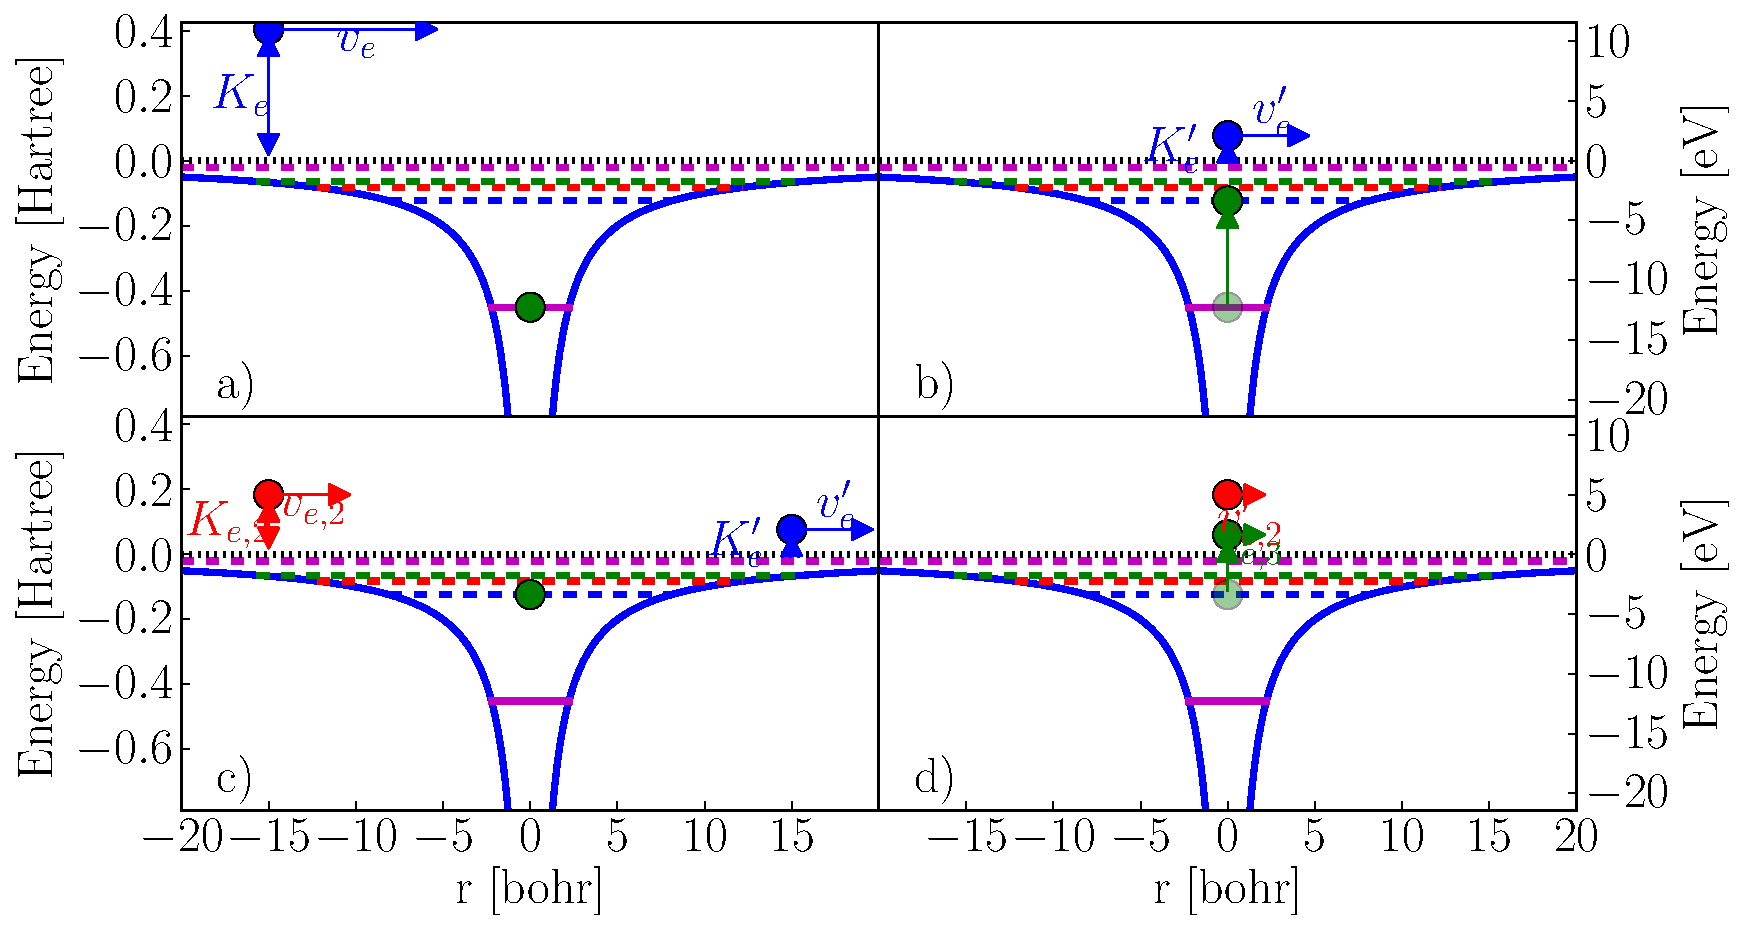
\includegraphics[width=\figurewidth]{figures/ionization_aci}
 \caption{ACI. First electron (in blue) collides with ion in a) and gives
          $K_e - K_e'$ of energy for the transition of a bound electron (in green)
          from the ground state in a) to an excited state in b). That first
          electron is thus slowed from $v_e$ in a) to $v_e'$ in b). A third electron
          (in red) collides with the ion in c) and gives the remaining kinetic
          energy required for the transition to continuum in d). The first step
          is a) to b) and the second step is from c) to d).}
 \label{fig:ionization:aci}
\end{figure}

% \begin{figure}
%  \centering
%     \begin{subfigure}{0.48\columnwidth}
%         \centering
%         \includegraphics[width=\textwidth]{figures/aci_0}
%         \caption{Before}
%         \label{fig:ionization:aci:0}
%     \end{subfigure}
%     \begin{subfigure}{0.48\columnwidth}
%         \centering
%         \includegraphics[width=\textwidth]{figures/aci_1}
%         \caption{1. }
%         \label{fig:ionization:aci:1}
%     \end{subfigure}
% \\
%     \begin{subfigure}{0.48\columnwidth}
%         \centering
%         \includegraphics[width=\textwidth]{figures/aci_2}
%         \caption{2. }
%         \label{fig:ionization:aci:2}
%     \end{subfigure}
%     \begin{subfigure}{0.48\columnwidth}
%         \centering
%         \includegraphics[width=\textwidth]{figures/aci_3}
%         \caption{3. }
%         \label{fig:ionization:aci:3}
%     \end{subfigure}
% \caption{ACI. First electron (in blue) gives $K_1$ energy for the transition
%           to an excited state. Second electron (in green) gives the remaining
%           $K_2$ necessary for the transition to continuum.}
% \label{fig:ionization:aci}
% \end{figure}


Figure \ref{fig:ionization:aci} shows an energy diagram of ACI and the
different transitions possible. This two-step model is implemented using
cross-sections for collisional transition (ground state to excited state and
excited state to continuum), similarly to traditional impact
ionization. See chapter \ref{section:intro:md:cross-sections} for more
details on cross-sections.

The ACI model revealed to be an important contribution to the field. As will be
seen from the publications, experimental results can be reproduced with this
model.



\subsubsection{Publications}

After the tools are presented in chapter \ref{section:tools}, the present thesis
consists of a series of four published articles and one article in preparation
where the models and tools are tested and used.


\subsubsubsection{ACI introduction paper}

First, the work on excited states and ACI in clusters was published in the article
``Augmented collisional ionization via excited states in XUV cluster
interactions'' published in 2011 in \textit{Journal of Physics B: Atomic,
Molecular and Optical Physics}\cite{Ackad2011a} and can be found in chapter
\ref{section:papers:aci} (page \pageref{section:papers:aci}). Argon clusters
(Ar$_{80}$ and Ar$_{147}$) were simulated with parameters used in experiments
at FLASH-DESY in 2008 by Bosted \textit{et al.}\cite{Bostedt2008}.
(32.8 nm -- 37.8 eV, 25 fs and intensities from $\ten{5}{13}$ to
$10^{14}$~W/cm$^{-2}$). It was found that not only could ACI explain the
Ar$^{4+}$ seen at FLASH but also that it
was a dominant process, happening more often than traditional impact ionization.
Due to the efficiency of ACI, high charge states can be reached in shorter time
than previously thought which can have a significant impact on biomolecules
imaging. This first ACI article was a stepping stone in the current work as it
showed the validity of the model, as simple as it could be.


\subsubsubsection{Cluster size influence}

Next, chapter \ref{section:papers:size} presents the article ``Clusters in
intense XUV pulses: Effects of cluster size on expansion dynamics and
ionization''. Also published in 2011 (\textit{Physical Review~A}\cite{Ackad2011b}),
argon clusters were simulated in the XUV regime (32.8 nm,
I~=~$\ten{5}{13}$~W/cm$^{2}$, 25 fs) with cluster sizes from Ar$_{55}$ to
Ar$_{2,057}$. It was found that the dynamics is highly collisional and
larger clusters even more so. By rapidly ionizing the lower charge states,
collisional processes will prevent photo-ionization even before the laser pulse
is finished. This mechanism was called \textit{collisionally reduced photoabsorption}.
The amount of energy absorbed through photo-ionization by Ar$_{55}$ clusters was
reduced by 30~\% and 45~\% by Ar$_{2,057}$ clusters when collisional processes
are included.
Higher charge states are more abundant and also appears sooner during the
dynamics in large clusters compared to smaller ones. ACI is vital for the
description; 20~\% of ions are in an excited state after the laser peak.
During the laser pulse, the distribution of charge inside clusters is
relatively isotropic but as the simulation evolves, the clusters' outer shells tend to
lose electrons more than the core and eventually disintegrate through Coulomb
explosion.
The core stays relatively neutral and expend thermodynamically.

The ion kinetic energy distribution revealed that Ar$^{2+}$  provided most of
the high energy tail. Additionally, the highest charge states had the least
energy. The highest charges states being created in the (neutral) core, the
electrons shield these high charge states, preventing them from accelerating
as much as the outer shells ions.

Electrons thermalize rapidly to a Maxwellian distribution. The larger clusters'
distribution are isotropic due to the high collisional rates while smaller
clusters keep the anisotropy coming from photoionization.



\subsubsubsection{Revisiting the 100 nm experiment}

Afterwards, chapter \ref{section:papers:100nm} contains the draft of the article
``Augmented Collisional Ionization in the VUV regime; a theoretical study''.
After Wabnitz \textit{et al.}'s
2002 DESY-FEL experiment's intensity was re-calibrated in 2010, we hypothesized
that our ACI model could still explain the high charge states seen in xenon
clusters, even with the lower intensities.
Since the VUV (98 nm, 12.65 eV)
photons cannot ionize a Xe$^{1+}$ to Xe$^{2+}$ (see table \ref{tab:ips} for xenon
ionization potentials), all charge states higher than Xe$^{1+}$ must be created
with other processes.
We included single photon ionization,
impact ionization, ACI and recombination in simulations of Xe$_{80}$ to Xe$_{5,083}$
interacting with DESY's 100~fs laser pulse at different intensities.
We compared our model
with previous work with ACI disabled and found good agreement.
The high performance of my
code implementation (see chapter \ref{section:tools:opencl} on GP-GPU) allowed
running thousands of MD simulations. The chaotic nature of the many-body
problem requires acquiring vast amount of data for valid statistics, giving more
weight to our results. On average, it was found that two more charge states are
accessible when ACI is enabled, a clear indication that ACI has a central role
amongst the ionization channels.

Due to the spatial intensity profile of the laser pulse, simulations were run
at different intensities to simulate the effect of experimental data acquired
from clusters dispersed in the laser's spatial profile. This improves the validity of
simulation data when comparing with experiments.
Our data was in good agreement with the 2002 experiment. Both the dominant
charge states and the highest charge states matched the experiment data. This
was not the case of other models which used the old intensity.

The last part of the article discuss the influence of the potential depth
of equation~\eqref{eqn:md:sigma}.
% Santra and Greene suggested\cite{Greene2003}
% using atomic potentials instead of a pure Coulombic one to explain the high
% charge states seen in experiments.
By allowing deeper potentials in our
simulations, it was hypothesized that larger charge states could be obtained.
The influence of the potential depth used in simulations is often neglected in
the literature. That article section sheds some light on the topic.
Since electrons are now allowed to go deeper in the ions potential well,
recombination must be used to prevent them from having a total energy less than
the ion's eigenvalues which would not be allowed quantum mechanically.



\subsubsubsection{Recombination }

Finally, chapter \ref{section:papers:recomb} present the article ``Recombination
effects in soft-x-ray cluster interactions at the xenon giant resonance''
published in May 2013 in New Journal of Physics.

Xenon atoms have, centred at around 13 nm (95.4 eV), a photoabsorption
cross-section approximately ten times larger for the 4d electrons than for the
outer-most shell 5p electrons; inner shell ionization is thus possible and
Auger processes creates highly charged ions, even in the case of xenon
gas\cite{Uiberacker2007}.

In experiments at 13.7 nm (90.5 eV) by Thomas \textit{et al.} in
2009\cite{Thomas2009}, the amount of Xe$^{1+}$ observed in clusters was
significantly more than in xenon gas, indicating that recombination effects were
important. At the time it was clear that photoabsorption and recombination alone
could not explain by itself these results.

Thomas \textit{et al.}'s experiment was described using our models. Xenon
clusters of sizes 147, 1,415 and 5,083 were simulated under a 13.7 nm
(90.5 eV) laser at different intensities from $\ten{1}{11}$ to
$\ten{5.8}{14}$ W/cm$^2$. Time-of-flight spectra were in good agreement with the
experiment. We also saw that the higher charge states came from the clusters'
outer-shells while the lower charged ions came from the clusters' core. Even
though ions in the neutral core can reach high charge states, they recombine
quickly to lower charge states. The expansion of ionized clusters is best
described by a Coulomb explosion of the outer-shells and a hydrodynamically
expending neutral core.



\subsubsubsection{A quantum approach}

Going further, interesting questions came up. For example, how is a bound
electron's wavefunction affected by a neighbouring ion or the cluster potential?
Due to my background in electromagnetic simulations, I was surprised to read
an article using the FDTD method -- normally used in electrodynamic simulations --
for quantum calculations. I was curious how far could the FDTD method be
applied to quantum problems and if it could answer some of our questions.
A QFDTD simulation package was thus developed, again from scratch,  implementing
two kinds of time evolution; real and imaginary. The model and its implementation details
are discussed in chapter \ref{section:tools:qfdtd}.

The work developed in chapter \ref{section:tools:qfdtd} was published in the article
``Nonlinear grid mapping applied to an FDTD-based, multi-center 3D
Schr\"odinger equation solver'' presented in chapter \ref{section:papers:qfdtd}.
Published in 2012 in \textit{Computer Physics Communications}\cite{Bigaouette2011}, it
explains the QFDTD method and its implementation, with emphasis on the new
nonlinear mapping introduced for faster calculation. The QFDTD package is the
first to use both the real and imaginary time evolution, opening the door to
easily get eigenvalues, eigenstates and their time evolution in a time-dependent
and arbitrary spacial shape potential.
The method was first validated by comparing with the analytic solutions of
the hydrogen atom and then applied to solve the H$_{2}^{+}$ molecule.
Comparison with experimental data was in good agreement for the eigenvalues
while the eigenstates could be visualize easily. A new method to calculate
eigenstates is also presented in the article. The publication also
describes in detail the nonlinear mapping that allows reducing both the memory
usage required to store the grid and the time required to calculate the time
evolution. The method is a generic way to obtain a nonuniform grid with cells
concentrated around multi-centres of interest for used in any (finite difference
based) partial differential equation solvers.

Before listing the different publication of the current thesis, the different
methodology and tools used and developed throughout the years will be presented
and discussed.


